% Created by tikzDevice version 0.10.1 on 2016-06-30 12:41:21
% !TEX encoding = UTF-8 Unicode
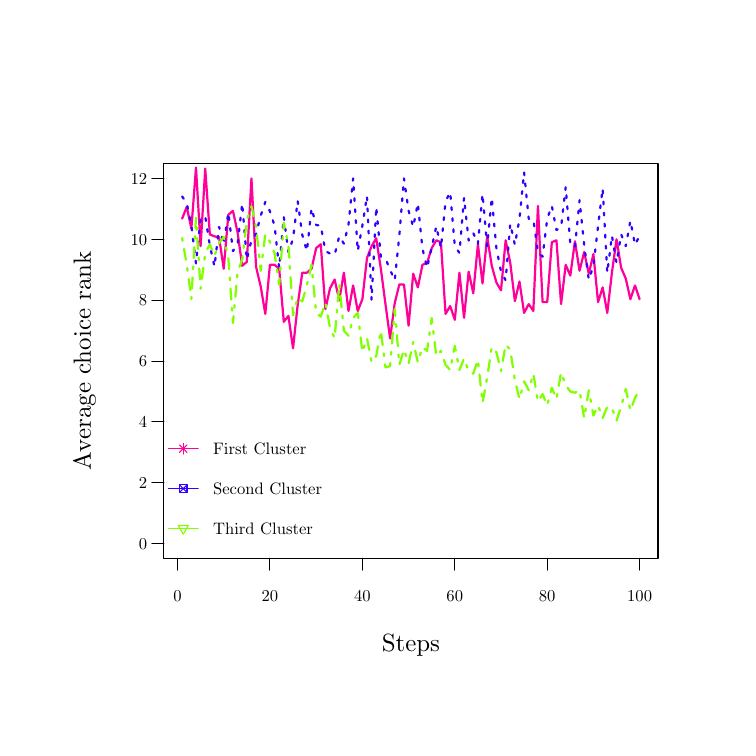
\begin{tikzpicture}[x=1pt,y=1pt]
\definecolor{fillColor}{RGB}{255,255,255}
\path[use as bounding box,fill=fillColor,fill opacity=0.00] (0,0) rectangle (252.94,252.94);
\begin{scope}
\path[clip] ( 49.20, 61.20) rectangle (227.75,203.75);
\definecolor{drawColor}{RGB}{255,0,153}

\path[draw=drawColor,line width= 0.8pt,line join=round,line cap=round] ( 55.81,183.92) --
	( 57.48,188.18) --
	( 59.15,180.37) --
	( 60.82,202.37) --
	( 62.49,173.98) --
	( 64.16,202.01) --
	( 65.83,178.24) --
	( 67.50,177.53) --
	( 69.17,177.18) --
	( 70.84,165.82) --
	( 72.51,185.34) --
	( 74.18,186.76) --
	( 75.85,178.95) --
	( 77.52,166.89) --
	( 79.19,168.31) --
	( 80.86,198.47) --
	( 82.53,166.53) --
	( 84.20,159.44) --
	( 85.87,149.50) --
	( 87.54,167.24) --
	( 89.21,167.24) --
	( 90.88,165.82) --
	( 92.55,146.66) --
	( 94.22,148.79) --
	( 95.89,137.08) --
	( 97.56,152.70) --
	( 99.23,164.40) --
	(100.90,164.40) --
	(102.57,165.82) --
	(104.24,173.27) --
	(105.91,174.69) --
	(107.58,151.28) --
	(109.25,158.73) --
	(110.92,161.92) --
	(112.59,154.47) --
	(114.26,164.40) --
	(115.93,150.57) --
	(117.60,159.79) --
	(119.27,150.57) --
	(120.94,154.82) --
	(122.61,169.73) --
	(124.28,173.98) --
	(125.95,176.82) --
	(127.62,165.82) --
	(129.29,153.05) --
	(130.96,140.63) --
	(132.63,153.41) --
	(134.30,160.15) --
	(135.97,160.15) --
	(137.64,145.25) --
	(139.31,164.05) --
	(140.98,159.08) --
	(142.65,167.24) --
	(144.32,167.95) --
	(145.99,173.27) --
	(147.66,176.11) --
	(149.33,175.40) --
	(151.00,149.50) --
	(152.67,152.34) --
	(154.34,147.37) --
	(156.01,164.40) --
	(157.68,148.08) --
	(159.35,164.76) --
	(161.02,156.95) --
	(162.69,174.69) --
	(164.36,160.50) --
	(166.03,177.53) --
	(167.70,166.89) --
	(169.37,160.86) --
	(171.04,158.02) --
	(172.71,176.11) --
	(174.38,167.95) --
	(176.05,154.12) --
	(177.71,161.21) --
	(179.38,149.86) --
	(181.05,153.05) --
	(182.72,150.57) --
	(184.39,188.53) --
	(186.06,153.76) --
	(187.73,153.76) --
	(189.40,175.40) --
	(191.07,176.11) --
	(192.74,153.05) --
	(194.41,167.24) --
	(196.08,163.34) --
	(197.75,175.76) --
	(199.42,165.11) --
	(201.09,171.86) --
	(202.76,164.05) --
	(204.43,171.15) --
	(206.10,153.76) --
	(207.77,159.08) --
	(209.44,149.86) --
	(211.11,164.40) --
	(212.78,176.47) --
	(214.45,166.18) --
	(216.12,162.28) --
	(217.79,154.82) --
	(219.46,159.79) --
	(221.13,154.82);
\end{scope}
\begin{scope}
\path[clip] (  0.00,  0.00) rectangle (252.94,252.94);
\definecolor{drawColor}{RGB}{0,0,0}

\path[draw=drawColor,line width= 0.4pt,line join=round,line cap=round] ( 54.14, 61.20) -- (221.13, 61.20);

\path[draw=drawColor,line width= 0.4pt,line join=round,line cap=round] ( 54.14, 61.20) -- ( 54.14, 56.92);

\path[draw=drawColor,line width= 0.4pt,line join=round,line cap=round] ( 87.54, 61.20) -- ( 87.54, 56.92);

\path[draw=drawColor,line width= 0.4pt,line join=round,line cap=round] (120.94, 61.20) -- (120.94, 56.92);

\path[draw=drawColor,line width= 0.4pt,line join=round,line cap=round] (154.34, 61.20) -- (154.34, 56.92);

\path[draw=drawColor,line width= 0.4pt,line join=round,line cap=round] (187.73, 61.20) -- (187.73, 56.92);

\path[draw=drawColor,line width= 0.4pt,line join=round,line cap=round] (221.13, 61.20) -- (221.13, 56.92);

\node[text=drawColor,anchor=base,inner sep=0pt, outer sep=0pt, scale=  0.60] at ( 54.14, 45.60) {0};

\node[text=drawColor,anchor=base,inner sep=0pt, outer sep=0pt, scale=  0.60] at ( 87.54, 45.60) {20};

\node[text=drawColor,anchor=base,inner sep=0pt, outer sep=0pt, scale=  0.60] at (120.94, 45.60) {40};

\node[text=drawColor,anchor=base,inner sep=0pt, outer sep=0pt, scale=  0.60] at (154.34, 45.60) {60};

\node[text=drawColor,anchor=base,inner sep=0pt, outer sep=0pt, scale=  0.60] at (187.73, 45.60) {80};

\node[text=drawColor,anchor=base,inner sep=0pt, outer sep=0pt, scale=  0.60] at (221.13, 45.60) {100};

\path[draw=drawColor,line width= 0.4pt,line join=round,line cap=round] ( 49.20, 66.48) -- ( 49.20,198.47);

\path[draw=drawColor,line width= 0.4pt,line join=round,line cap=round] ( 49.20, 66.48) -- ( 44.92, 66.48);

\path[draw=drawColor,line width= 0.4pt,line join=round,line cap=round] ( 49.20, 88.48) -- ( 44.92, 88.48);

\path[draw=drawColor,line width= 0.4pt,line join=round,line cap=round] ( 49.20,110.47) -- ( 44.92,110.47);

\path[draw=drawColor,line width= 0.4pt,line join=round,line cap=round] ( 49.20,132.47) -- ( 44.92,132.47);

\path[draw=drawColor,line width= 0.4pt,line join=round,line cap=round] ( 49.20,154.47) -- ( 44.92,154.47);

\path[draw=drawColor,line width= 0.4pt,line join=round,line cap=round] ( 49.20,176.47) -- ( 44.92,176.47);

\path[draw=drawColor,line width= 0.4pt,line join=round,line cap=round] ( 49.20,198.47) -- ( 44.92,198.47);

\node[text=drawColor,anchor=base east,inner sep=0pt, outer sep=0pt, scale=  0.60] at ( 43.20, 64.41) {0};

\node[text=drawColor,anchor=base east,inner sep=0pt, outer sep=0pt, scale=  0.60] at ( 43.20, 86.41) {2};

\node[text=drawColor,anchor=base east,inner sep=0pt, outer sep=0pt, scale=  0.60] at ( 43.20,108.41) {4};

\node[text=drawColor,anchor=base east,inner sep=0pt, outer sep=0pt, scale=  0.60] at ( 43.20,130.41) {6};

\node[text=drawColor,anchor=base east,inner sep=0pt, outer sep=0pt, scale=  0.60] at ( 43.20,152.40) {8};

\node[text=drawColor,anchor=base east,inner sep=0pt, outer sep=0pt, scale=  0.60] at ( 43.20,174.40) {10};

\node[text=drawColor,anchor=base east,inner sep=0pt, outer sep=0pt, scale=  0.60] at ( 43.20,196.40) {12};

\path[draw=drawColor,line width= 0.4pt,line join=round,line cap=round] ( 49.20, 61.20) --
	(227.75, 61.20) --
	(227.75,203.75) --
	( 49.20,203.75) --
	( 49.20, 61.20);
\end{scope}
\begin{scope}
\path[clip] (  0.00,  0.00) rectangle (252.94,252.94);
\definecolor{drawColor}{RGB}{0,0,0}

\node[text=drawColor,anchor=base,inner sep=0pt, outer sep=0pt, scale=  0.90] at (138.47, 27.60) {Steps};

\node[text=drawColor,rotate= 90.00,anchor=base,inner sep=0pt, outer sep=0pt, scale=  0.90] at ( 22.80,132.47) {Average choice rank};
\end{scope}
\begin{scope}
\path[clip] ( 49.20, 61.20) rectangle (227.75,203.75);
\definecolor{drawColor}{RGB}{51,0,255}

\path[draw=drawColor,line width= 0.8pt,dash pattern=on 1pt off 3pt ,line join=round,line cap=round] ( 55.81,191.96) --
	( 57.48,189.49) --
	( 59.15,181.41) --
	( 60.82,167.71) --
	( 62.49,184.10) --
	( 64.16,184.77) --
	( 65.83,174.22) --
	( 67.50,166.59) --
	( 69.17,180.96) --
	( 70.84,174.67) --
	( 72.51,186.12) --
	( 74.18,172.20) --
	( 75.85,174.67) --
	( 77.52,189.49) --
	( 79.19,169.06) --
	( 80.86,176.24) --
	( 82.53,178.49) --
	( 84.20,185.00) --
	( 85.87,189.94) --
	( 87.54,186.57) --
	( 89.21,181.41) --
	( 90.88,166.14) --
	( 92.55,184.55) --
	( 94.22,171.75) --
	( 95.89,176.69) --
	( 97.56,190.38) --
	( 99.23,178.04) --
	(100.90,172.20) --
	(102.57,187.69) --
	(104.24,181.63) --
	(105.91,181.41) --
	(107.58,172.20) --
	(109.25,171.31) --
	(110.92,170.86) --
	(112.59,177.59) --
	(114.26,174.90) --
	(115.93,181.86) --
	(117.60,198.47) --
	(119.27,172.20) --
	(120.94,181.41) --
	(122.61,192.18) --
	(124.28,154.47) --
	(125.95,188.14) --
	(127.62,170.18) --
	(129.29,169.51) --
	(130.96,165.47) --
	(132.63,161.65) --
	(134.30,177.81) --
	(135.97,198.47) --
	(137.64,186.79) --
	(139.31,180.96) --
	(140.98,189.49) --
	(142.65,173.10) --
	(144.32,166.14) --
	(145.99,173.55) --
	(147.66,181.18) --
	(149.33,173.33) --
	(151.00,190.16) --
	(152.67,193.53) --
	(154.34,174.00) --
	(156.01,171.53) --
	(157.68,191.51) --
	(159.35,176.02) --
	(161.02,178.71) --
	(162.69,174.90) --
	(164.36,192.85) --
	(166.03,174.00) --
	(167.70,191.51) --
	(169.37,173.33) --
	(171.04,164.80) --
	(172.71,161.65) --
	(174.38,182.08) --
	(176.05,174.45) --
	(177.71,183.88) --
	(179.38,200.71) --
	(181.05,183.88) --
	(182.72,183.65) --
	(184.39,171.98) --
	(186.06,170.18) --
	(187.73,183.88) --
	(189.40,188.59) --
	(191.07,179.83) --
	(192.74,180.73) --
	(194.41,195.32) --
	(196.08,174.90) --
	(197.75,173.55) --
	(199.42,190.61) --
	(201.09,174.45) --
	(202.76,161.88) --
	(204.43,166.82) --
	(206.10,181.18) --
	(207.77,194.87) --
	(209.44,164.35) --
	(211.11,177.81) --
	(212.78,167.94) --
	(214.45,178.26) --
	(216.12,174.00) --
	(217.79,183.20) --
	(219.46,174.45) --
	(221.13,177.81);
\definecolor{drawColor}{RGB}{128,255,0}

\path[draw=drawColor,line width= 0.8pt,dash pattern=on 1pt off 3pt on 4pt off 3pt ,line join=round,line cap=round] ( 55.81,176.93) --
	( 57.48,167.30) --
	( 59.15,154.93) --
	( 60.82,184.26) --
	( 62.49,158.59) --
	( 64.16,171.43) --
	( 65.83,174.63) --
	( 67.50,170.51) --
	( 69.17,175.09) --
	( 70.84,177.38) --
	( 72.51,169.59) --
	( 74.18,146.22) --
	( 75.85,164.55) --
	( 77.52,169.14) --
	( 79.19,183.34) --
	( 80.86,188.38) --
	( 82.53,181.05) --
	( 84.20,165.01) --
	( 85.87,178.30) --
	( 87.54,175.55) --
	( 89.21,171.43) --
	( 90.88,159.97) --
	( 92.55,182.43) --
	( 94.22,174.18) --
	( 95.89,148.97) --
	( 97.56,155.39) --
	( 99.23,154.01) --
	(100.90,159.97) --
	(102.57,167.30) --
	(104.24,149.89) --
	(105.91,148.51) --
	(107.58,153.55) --
	(109.25,144.39) --
	(110.92,140.72) --
	(112.59,160.43) --
	(114.26,143.47) --
	(115.93,141.64) --
	(117.60,148.05) --
	(119.27,149.89) --
	(120.94,135.68) --
	(122.61,140.72) --
	(124.28,132.01) --
	(125.95,134.31) --
	(127.62,143.47) --
	(129.29,130.18) --
	(130.96,130.64) --
	(132.63,151.26) --
	(134.30,131.10) --
	(135.97,136.60) --
	(137.64,131.56) --
	(139.31,139.35) --
	(140.98,132.01) --
	(142.65,137.51) --
	(144.32,136.14) --
	(145.99,148.05) --
	(147.66,134.31) --
	(149.33,136.14) --
	(151.00,131.10) --
	(152.67,129.26) --
	(154.34,137.97) --
	(156.01,129.26) --
	(157.68,133.39) --
	(159.35,128.81) --
	(161.02,127.89) --
	(162.69,132.93) --
	(164.36,117.35) --
	(166.03,126.51) --
	(167.70,137.51) --
	(169.37,135.68) --
	(171.04,128.81) --
	(172.71,138.43) --
	(174.38,136.60) --
	(176.05,125.60) --
	(177.71,118.72) --
	(179.38,125.14) --
	(181.05,121.93) --
	(182.72,127.89) --
	(184.39,117.81) --
	(186.06,120.56) --
	(187.73,116.43) --
	(189.40,122.85) --
	(191.07,118.72) --
	(192.74,128.35) --
	(194.41,123.77) --
	(196.08,121.47) --
	(197.75,121.02) --
	(199.42,121.93) --
	(201.09,111.85) --
	(202.76,121.93) --
	(204.43,112.77) --
	(206.10,116.43) --
	(207.77,111.85) --
	(209.44,115.97) --
	(211.11,115.52) --
	(212.78,110.93) --
	(214.45,115.97) --
	(216.12,122.39) --
	(217.79,114.60) --
	(219.46,119.18) --
	(221.13,121.93);
\definecolor{drawColor}{RGB}{255,0,153}

\path[draw=drawColor,line width= 0.4pt,line join=round,line cap=round] ( 50.82,100.80) -- ( 61.62,100.80);
\definecolor{drawColor}{RGB}{51,0,255}

\path[draw=drawColor,line width= 0.4pt,line join=round,line cap=round] ( 50.82, 86.40) -- ( 61.62, 86.40);
\definecolor{drawColor}{RGB}{128,255,0}

\path[draw=drawColor,line width= 0.4pt,line join=round,line cap=round] ( 50.82, 72.00) -- ( 61.62, 72.00);
\definecolor{drawColor}{RGB}{255,0,153}

\path[draw=drawColor,line width= 0.4pt,line join=round,line cap=round] ( 54.87, 99.45) -- ( 57.57,102.15);

\path[draw=drawColor,line width= 0.4pt,line join=round,line cap=round] ( 54.87,102.15) -- ( 57.57, 99.45);

\path[draw=drawColor,line width= 0.4pt,line join=round,line cap=round] ( 54.31,100.80) -- ( 58.13,100.80);

\path[draw=drawColor,line width= 0.4pt,line join=round,line cap=round] ( 56.22, 98.89) -- ( 56.22,102.71);
\definecolor{drawColor}{RGB}{51,0,255}

\path[draw=drawColor,line width= 0.4pt,line join=round,line cap=round] ( 54.87, 85.05) rectangle ( 57.57, 87.75);

\path[draw=drawColor,line width= 0.4pt,line join=round,line cap=round] ( 54.87, 85.05) -- ( 57.57, 87.75);

\path[draw=drawColor,line width= 0.4pt,line join=round,line cap=round] ( 54.87, 87.75) -- ( 57.57, 85.05);
\definecolor{drawColor}{RGB}{128,255,0}

\path[draw=drawColor,line width= 0.4pt,line join=round,line cap=round] ( 56.22, 69.90) --
	( 58.04, 73.05) --
	( 54.40, 73.05) --
	( 56.22, 69.90);
\definecolor{drawColor}{RGB}{0,0,0}

\node[text=drawColor,anchor=base west,inner sep=0pt, outer sep=0pt, scale=  0.60] at ( 67.02, 98.73) {First Cluster};

\node[text=drawColor,anchor=base west,inner sep=0pt, outer sep=0pt, scale=  0.60] at ( 67.02, 84.33) {Second Cluster};

\node[text=drawColor,anchor=base west,inner sep=0pt, outer sep=0pt, scale=  0.60] at ( 67.02, 69.93) {Third Cluster};
\end{scope}
\end{tikzpicture}
